\clearpage
\chapter[Workflow management]{Workflow management\\- A new approach for research data and metadata management}
\label{sec:workflows}
The long process that starts from the generation of data, and ends in a scientific publication, can be separated into many individual steps. These subdivision may be coarse, like the separation only of experiment and subsequent analysis. Or they may be very fine, as each individual operation, and substeps within, may constitute and be implemented in independent processes.

Workflow management is the concept to organize these individual steps. The granularity of the steps to manage highly depends on the complexity of the tasks and the diversity of the processing steps. A common and generic example forming such a workflow management system (WMS) is a queuing system used in cluster computing such as \software{slurm}\footnote{slurm workload manager, \url{https://slurm.schedmd.com/}} or  \software{torque}\footnote{torque resource manager, \url{http://www.adaptivecomputing.com/products/torque/}} and \software{maui}\footnote{maui cluster scheduler, \url{http://www.adaptivecomputing.com/products/maui/}}. Here users submit a number of, in the simplest case, independent jobs (computing steps) which are then scheduled and distributed to suitable compute resources depending on the requested and available resources. This is a simple example, because the individual processing steps typically do not depend on each other and only the required amount of resources and time needs to be taken into account when organizing the execution. Already with these systems, it is possible to implement more complex scenarios, e.g. by defining an order of execution via dependency statements for individual jobs.

In this chapter we apply the concept of workflow management to solve the data and metadata management issues identified in \cref{sec:scidata_shortcomings}. A systematic workflow approach for data and metadata management supports the rigorous implementation of the FAIR principles, since the automation of processing steps relies to some extend on FAIR principles, i.e data should to have a unique identifier and should be organized in a structured fashion using standardized tools. Additionally, the implementation of a data and metadata workflow increases the reproducibility of the processing steps, as these are documented and provenance information can be tracked for each step of the workflow. Workflow management is suited to tackle the issues we identified in \cref{sec:scidata_shortcomings}, since it is designed to coordinate interdependent steps of a process as they occur in the data and metadata pipeline of the Reach-to-Grasp project. In the following, we present available WMSs and identify requirements for the applicability in the context of scientific projects in general as well as for Reach-to-Grasp and similar projects in particular.

For scientific projects like the Reach-to-Grasp experiment described in \cref{sec:data} there are dependencies between individual steps of the process from data acquisition to publication (see \cref{fig:scidata_metadata_pipeline,fig:scidata_reachgraspio_diagram}). The workflow management concept has been applied in a number of scientific fields like genomics or imaging data. In these fields a systematic approach to data processing and analysis is required and feasible, since they are dealing with large and numerous datasets which exceed manual monitoring or processing power \citep[e.g.][]{Palm_2010}.
For these and other disciplines, there are a number of platforms and tools available to implement pre \& post processing as well as analysis processing steps: Galaxy\footnote{Galaxy, \url{https://galaxyproject.org}, RRID:SCR\_006281}, an  open, web-based platform providing bioinformatics tools and services for data intensive genomics research; VisTrails\footnote{VisTrails, \url{https://www.vistrails.org}, RRID:SCR\_006261}, an open-source scientific workflow and provenance management system that provides support for simulations, data exploration and visualization; Taverna\footnote{Taverna, \url{https://taverna.incubator.apache.org}, RRID:SCR\_004437}, a scalable, open source \& domain independent tool for designing and executing workflows;  GenePattern\footnote{GenePattern, \url{http://www.broadinstitute.org/cancer/software/genepattern}, RRID:SCR\_003201}, a genomics analysis platform that provides access to hundreds of tools for gene expression analysis, SNP analysis, flow cytometry, RNA-seq analysis, and common data processing tasks; Renku\footnote{Renku, \url{https://datascience.ch/renku}}, an online software platform for reproducible and collaborative data science including workflow management aspects; Terra\footnote{\url{https://terra.bio/}}, a scalable platform  for biomedical research for data analysis and collaboration; Ugene \citep{Okonechnikov_2012} a multi platform open-source software for molecular biology; Luigi\footnote{Luigi, \url{https://luigi.readthedocs.io}}, a Python based tool for building complex pipelines of batch jobs; Airflow \footnote{Airflow, \url{https://airflow.apache.org/index.html}}, a platform programmatically author, schedule and monitor workflows; pinball\footnote{pinball, \url{https://github.com/pinterest/pinball}}, a scalable workflow manager with scheduling capability implemented in JavaScript and Python; make, a basic build automation tool available since 1976 with multiple implementations (e.g. gnumake\footnote{gnumake, \url{https://www.gnu.org/software/make/}}) and snakemake\footnote{Snakemake, \url{https://snakemake.readthedocs.io/en/stable/}, RRID:SCR\_003475}, a Python based language and execution environment for make-like workflows. 

In simple and straightforward projects, one may use plain bash scripts to coordinate the sequential execution of the individual steps of a workflows, mimicking a WMS. However, once the situations grows more complex, the same issues arise as discussed for the Reach-to-Grasp metadata pipeline (\cref{sec:scidata_shortcomings}): the bash script would form a monolithic script, trying to cover all possible dependencies between individual scripts resulting in overly complex code. Additionally, the script could only be executed all at once, without taking into account which steps of the workflow are actually required due to updates in the underlying sources files.

Scientific projects, such as the Reach-to-Grasp project presented in \cref{sec:data}, can benefit greatly from a structured workflow approach. However, the development of the workflow should in the best case smoothly integrate with the existing scientific tools and approaches used in the project. In the following, we discuss a number of essential features of a WMS, which are generally required in scientific projects. The WMS should 
\begin{quote}
\begin{description}
 \setlength{\itemsep}{5pt}
 \setlength{\parskip}{0pt}
 \setlength{\parsep}{0pt}
 \item[slim] not introduce unnecessary additional computational overhead
 \item[easy]  not require expert knowledge to implement and configure a workflow
 \item[standalone] not introduce additional unnecessary dependencies to other projects and programming languages
  \item[visual] be able to generate a visual overview of the workflow for inspection and debugging purposes
  \item[debuggable] be easy to debug
  \item[active] be actively supported
  \item[open] be open source and freely available\\
\end{description}
\end{quote}
Furthermore, we identify additional, more specific requirements in the context of the Reach-to-Grasp and similar projects. Here, the WMS should
\begin{quote}
\begin{description}
 \setlength{\itemsep}{5pt}
 \setlength{\parskip}{0pt}
 \setlength{\parsep}{0pt}
 \item[Python] inherently support Python as many of the existing scripts are implemented in Python
 \item[integration] integrate well with existing scripts as the existing code base should not depend on the WMS.
 \item[flexibility] provide the flexibility to implement processing steps based on bash (for usage of external tools, e.g. for spike sorting)
 \item[HPC] support local workflow execution as well as the usage of compute clusters by supporting common queuing systems
\end{description}
\end{quote}

The general requirements for a slim and standalone WMS with only minimal overhead already excludes the majority of WMSs listed above as these provide a multitude of features like web applications that are not required in the context of the scientific projects presented here. This rules out Galaxy, Renku, Terra as these are web based WMSs based on a webinterface for user interaction. Ugene and GenePattern focus on very different domains (molecular biology \& genomics, respectively) and provide a multitude of tools for these domains, which are not required here. Pinball and Taverna are java based which is not used in the context of the Reach-to-Grasp or related projects.  In addition, Taverna is a highly developed workflow system with 3500 services available, which surpasses our requirements. Airflow and Luigi are Python-based WMSs that rely on a custom workflow definition in a Python script, which requires tool-specific knowledge for implementation and maintenance of the workflow. VisTrails is Python based as well, but relies on a graphical user interface for the workflow definition, thereby making the implementation of complex workflows cumbersome. Make is a well established tool for the organization of build processes and is therefore available on all operating systems. It has been shown that scientific workflows for quality assurance can be implemented using make \citep{Askren_2016}. However, the workflow definition via make is laborious as well due to a limited utility functionality. Here, snakemake offers a hybrid solution of make and Python. The workflow definition is implemented in a make concept, but Python functionality can be used to facilitate the definition of the workflow within the rigid structure provided by make. Since Python is already the language of choice in the Reach-to-Grasp project, snakemake does not introduce any additional language dependencies and is therefore our tool of choice in order to demonstrate the usage of WMSs in the context of data and metadata management in scientific projects.


\section{Workflow management tools - Snakemake}
\label{sec:snakemake}
In this section we discuss snakemake as a WMS, as it is domain independent, slim and easily integrates with Python based projects, e.g. to the Reach-to-Grasp and related projects (\cref{sec:data}).

Snakemake is a generic workflow management tool derived from the build automation tool make combined with Python features \citep{Koster_2012}. It is available as bioconda\footnote{\url{https://anaconda.org/bioconda/snakemake}} and PyPi package\footnote{\url{https://pypi.org/project/snakemake}}. We consider the so far latest version $5.5.4$ here.

We demonstrate the basic features of snakemake based on two minimal workflow examples. The first one (\cref{code:workflows_simple_snakefile}) demonstrates the basic concept of make and the ability of snakemake to define steps in the workflow in which the involved filenames are not known beforehand. The second, more complex workflow (\cref{code:workflows_python_snakefile}) demonstrates the integration of snakemake with Python and showcases its capabilities of flexibly deducing rule dependencies and parameters of individual workflow steps.

The description of individual steps of a workflow within snakemake is closely related to Make: A processing step is defined via its input and output files (\cref{code:workflows_simple_snakefile}, line 11 and 12). The core of a rule is the instruction how to generate the output files based on the input files. Here snakemake offers multiple options based on direct execution of Python scripts or bash scripting. Bash scripts offer the most flexibility and are marked with the \code{shell} keyword (\cref{code:workflows_simple_snakefile}, line 13). Within executed shell command references to the input and output files can be used via Python based reformatting of the command before execution. E.g. in \cref{code:workflows_simple_snakefile}, line 13 the filename specified by the input of the rule \code{simple\_copy\_rule} (line 11) is automatically copied to the filename specified by the output of the rule by using \code{\{input\}} and \code{\{output\}} in the shell command. The same concept can be used to formulate snakemake rules in a more flexible fashion. E.g. in \cref{code:workflows_simple_snakefile} a set of flexible rules is introduced, which use an additional wildcard \code{\{filename\}} to be able to generate and copy not only files with filename \code{'file.md'}, but any markdown file. Here, the value of the variable \code{\{filename\}} is only determined during the execution of the workflow. Therefore, the same rule can be used multiple times within a workflow with different wildcard parameters. Hereby, the value of the wildcard is determined recursively by the required output file.

The dependencies between snakemake rules are evaluated based on required files. By default snakemake uses the first rule within a \code{Snakefile} as main rule and tries to execute this rule. Alternatively snakemake can be called with a filename as an argument. In this case snakemake attempts to build the requested file based on all available rules, thereby matching in and output files of rules and checking the availability of basic input files. For this purpose snakemake generates an acyclic directed graph of rule dependencies (e.g. see \cref{fig:python_demo}) and infers all wildcard parameters from this. In case multiple rules can be used for generation of the same file a rule priority order can be be defined (\cref{code:workflows_simple_snakefile}, lines 1-3). Snakemake only executes rules and creates or overwrites files if the output files of a rule do not exist or the input files have a more recent modification time stamp than the output files. This guarantees that the output files of a snakemake workflow are always based on the most recent version of input files and at the same time minimizes the computational overhead, since only required or outdated files are generated.


\begin{codeenv}
\textbf{Snakemake header}
\inputminted[firstline=1, lastline=3, linenos,tabsize=2,breaklines, fontsize=\scriptsize]{bash}{figures/workflows/simple_demo.snakefile}
\begin{multicols}{2}
\textbf{Simple rules}
\inputminted[firstline=5, lastline=13, linenos,tabsize=2,breaklines, fontsize=\scriptsize]{bash}{figures/workflows/simple_demo.snakefile}
\columnbreak
\textbf{Flexible rules}
\inputminted[firstline=15, lastline=23, linenos,tabsize=2,breaklines, fontsize=\scriptsize]{bash}{figures/workflows/simple_demo.snakefile}
\end{multicols}
\caption[Minimal snakemake example workflow]{Minimal snakemake example workflow. The workflow consists of two rules: i) generation of a markdown file (.md) and ii) conversion to a text file by plain copy of the content into a file with .txt extension. Two versions of each rule are implemented, demonstrating snakemake features at different complexities: The simple version of the rule handles filenames explicitly (left), whereas the flexible version of the rule is using wildcards to handle filenames (right). To resolve ambiguities between the two versions of the rules, we define a rule priority order in the first lines of the snakemake file.}
\label[codelisting]{code:workflows_simple_snakefile}
\end{codeenv}


\begin{codeenv}
\begin{multicols}{2}
\textbf{Snakefile}\\
\inputminted[firstline=1, lastline=40, linenos,tabsize=2,breaklines, fontsize=\scriptsize]{bash}{figures/workflows/python_demo.snakefile}
\columnbreak
\textbf{Environments}\\
\textbf{plotting\_environment.yaml}
\inputminted[linenos,tabsize=2,breaklines, fontsize=\scriptsize]{yaml}{figures/workflows/envs/plotting_environment.yaml}
\textbf{data\_generation\_environment.yaml}
\inputminted[linenos,tabsize=2,breaklines, fontsize=\scriptsize]{yaml}{figures/workflows/envs/data_generation_environment.yaml}
\textbf{config.yaml}
\inputminted[linenos,tabsize=2,breaklines, fontsize=\scriptsize]{yaml}{figures/workflows/config.yaml}
\end{multicols}
\caption[Snakemake example workflow for data generation and plotting]{Snakemake example workflow for data generation and plotting. The workflow consists of three rules, for data generation, data visualization and specification of the all output files of the workflow. The first two rules can be executed in dedicated conda environments, specified via the \code{conda}-directive and are shown on the right. The workflow uses a configuration file (Snakefile, line 1, \code{config.yaml}), specifying the format for storing \software{Neo} structures. This specification is also used to provide a constraint for wildcards with the name \code{data\_ext}, which resolves ambiguities between the data generation and visualization rule. The rule \code{all} is by default executed when snakemake is run. It specifies two required output formats of the workflow. For the visualization of the workflow diagram when running the \code{all} rule, see \cref{fig:python_demo}.}
\label[codelisting]{code:workflows_python_snakefile}
\end{codeenv}


Snakemake rules can be executed in dedicated, containerized environments. For Python workflows, snakemake supports conda environments on a per-rule level. Here, the conda environment can be defined via a \code{yaml} file specifying the conda (and PyPi) dependencies (see \cref{code:workflows_python_snakefile} Snakefile, line 16 and 23 and environments). When no cached version of the environment exists or the \code{yaml} environment definition was updated, snakemake builds the environment using conda.

\cref{code:workflows_python_snakefile} demonstrates a more complex workflow using two generic Python scripts (\cref{code:workflows_python_scripts}) . The first script generates data based on the \software{Neo} package, whereas the second script visualizes any data accessible via \software{Neo} using the Python \software{Matplotlib} package. These scripts are implemented to be used as standalone scripts, and require arguments from the command line indicating the filename. Additionally, they do not rely on a fixed data file format, but support any format supported by the  \software{Neo} framework. This, in combination with the explicit definition of the required conda environments in form of \code{yaml} files makes the scripts highly flexible and generic, such that they can be easily reused in different contexts and projects. Furthermore, the snakemake implementation of the workflow keeps the generality of the code by providing flexibility in the used data format, which is defined via an additional configuration \code{yaml} file, and the usage of wildcards for flexible handling of filenames. The resulting snakemake workflow as well as the output visualization of the randomly generated data can be seen in \cref{fig:python_demo}.

\begin{figure}
%     \begin{multicols}{2}
    \begin{minipage}[t]{0.4\textwidth}
    \textbf{A}\\
    \includesvg[width=\textwidth, pretex=\relscale{0.8}]{figures/workflows/python_demo_escus}
    \end{minipage}
    \begin{minipage}[t]{0.6\textwidth}
%     \columnbreak\\
    \textbf{B}\\
    \includesvg[width=\textwidth]{figures/workflows/data}\\
    \end{minipage}
    %     \end{multicols}
 \caption[Snakemake example workflow for data generation and plotting]{Snakemake example workflow for data generation and plotting. The workflow diagram (A) and resulting plot (B). The workflow consists of two rules of which the \code{plot\_data} rule is executed twice with different parameters to generate the final plot in two file formats (\code{ext:svg}, \code{ex:png}, respectively). Different rules are color coded and the rule name is indicated at the top of each node.  The command line parameters of the scripts are indicated below the rule name. The frame style (solid/dashed) indicates if this rule needs to be run to generate a final output file. In this example, the data file was already generated, wherefore snakemake would not rerun this rule unnecessarily (dashed box). The arrows indicate the dependencies between the rule executions. Rules at the top need to be executed first, since they generate output files that are required as input for the subsequent rules executions.}
\label{fig:python_demo}
\end{figure}


\begin{codeenv}
\begin{multicols}{2}
\textbf{Data generation}
\inputminted[linenos,tabsize=2,breaklines, fontsize=\scriptsize]{python}{figures/workflows/generate_data.py}
\columnbreak
\textbf{Data visualization}
\inputminted[linenos,tabsize=2,breaklines, fontsize=\scriptsize]{python}{figures/workflows/plot_data.py}
\end{multicols}
\caption[Standalone Python scripts used in \cref{code:workflows_python_snakefile}]{Standalone Python scripts used in \cref{code:workflows_python_snakefile}. The two scripts for data generation and visualization contain generic functions, relying on command line parameters to provide the arguments for the function calls (lines 21-24 and lines 18-21, respectively). The \textbf{data generation} is split into two functions, one for generation of the \software{Neo} structure (\code{generate\_neo\_data}) and one for saving the \software{Neo} structure to disc (\code{save\_neo\_block}). The first function generates a \software{Neo} \code{Block} containing a single \code{AnalogSignal} with randomly generated data (lines 4-12). The second function receives a generic \software{Neo} \code{Block} and saves it in the format specified by the provided filename (lines 16-19). If the script is executed from the command line, the input parameter \code{filename} is extracted from the command line arguments and both functions are executed consecutively, passing the \software{Neo} \code{Block} from one function the next (lines 21-24). The \textbf{data visualization} uses the same concept as the data generation. Here the two internal functions are loading a \software{Neo} block from the specified data source filename (\code{load\_neo\_block}, lines 4-7) and visualize the first \code{AnalogSignal} of a given plot, saving the result in a requested filename (\code{plot\_analogsignal}, lines 9-16). Both functions are called if the script is called from the command line and the two parameters specifying the data location as well as the output plot filename are extracted from the command line arguments.
}
\label[codelisting]{code:workflows_python_scripts}
\end{codeenv}

In addition to the features demonstrated in the example scripts, snakemake integrates well distributed storage concepts, such as Google Cloud Storage\footnote{Google Cloud Storage, \url{https://cloud.google.com/storage/}}, Dropbox\footnote{Dropbox, \url{https://www.dropbox.com}}, or the secure shell protocol (SSH). Remote file sources are declared in the header of the snakemake file and individual files can be referenced from these sources in the same manner as local files. Besides access to remote files, snakemake also integrates with high-performance compute clusters by supporting common queuing systems such as the slurm workload manager\footnote{slurm, \url{https://slurm.schedmd.com}}. Here, a configuration file can be used to specify the cluster job parameters on a rule-level, permitting detailed resource management.

\paragraph{Summary}
We presented the application of basic snakemake features based on two examples demonstrating the modularization of a workflow into individual rules and their file-based dependency handling. We highlighted the flexibility of this approach by introducing wildcard based filename handling and explained the snakemake dependency graph. We provided examples of generic standalone Python scripts for seamless integration into snakemake rules and demonstrated advanced configuration features of the workflow via additional configuration files and wildcard constraints. We introduced additional features for integration of remote files and cluster usage.
The presented features make snakemake our tool of choice for the implementation of scientific workflows, as it provides a domain-independent and slim option for workflow definition which integrates well with existing scripted data processing steps.


\section{Practical application}
Snakemake has been applied in a variety of fields and projects. Many of the provided examples and tutorials are set in the field of genomics\footnote{\url{https://snakemake.readthedocs.io/en/stable/getting_started/examples.html}}$^,$\footnote{\url{https://snakemake.readthedocs.io/en/stable/tutorial/basics.html}}. Here we present a workflow design in the context of the Vision-for-Action project, a successor project of Reach-to-Grasp.

\subsection{The Vision-for-Action project}
The Vision-For-Action project builds on top of the Reach-to-Grasp project as it extends the investigation of motor control only to the interaction of motor and visual activity. The involved continuous integration of both visual input and motor control demand a more sophisticated experimental task protocol. The experimental hardware is a Real-time visuomotor behavior and electrophysiology recording (RIVER) setup, which utilizes a \software{Blackrock} system in order to record neuronal activity, as described for the Reach-to-Grasp experiment (\cref{sec:data}). For more details, we refer to \citet{deHaan_2018,deHaan_2018a}. The recording system additionally encompasses an eye tracking as well as a hand movement control system and a complex task design, which includes the sequential pointing to up to six targets. To the current date, only a single monkey was recorded in the Vision-for-Action setup.

\paragraph{The task}
In the Vision-for-Action experiment a monkey is positioned in front of a horizontal, semi-transparent mirror, onto which a white dot corresponding to its hand position below the mirror, is projected (\cref{fig:river_setup}). The monkey is trained to initialize a task by moving the hand cursor into the area of a central, illuminated target. After a waiting period of $200ms$, during which the monkey has to stay in the center, the central target is deactivated and, depending on the task type, one or multiple of 6 peripheral targets are illuminated. To receive a reward, the monkey has to deactivate all illuminated targets by moving the hand cursor into the each of the targets. Depending on the task additional targets appear upon the deactivation of a previous one. Two classic task types are currently implemented: The landing task, in which the monkey is presented a sequence of three peripheral targets, which he has to deactivate by staying in each of the targets for $100ms$ resulting in mostly straight hand movements to the target. In the drawing task, the monkey is presented multiple targets at once and can chose an order and route to deactivate these. In this task type the monkey only needs to touch the target with the hand cursor. It was observed that this typically causes very curved hand movement trajectories.


\paragraph{The setup}
The RIVER setup consists of three components recording different modalities: i) the neural activity via a \software{Blackrock} system described in the context of the Reach-to-Grasp experiment ii) the eye movement via a an EyeLink tracking system and iii) the arm movement via a Kinarm motorized exoskeleton (\cref{fig:river_setup}).

As in the Reach-to-Grasp experiment, neural activity is recorded using a Utah array recording device. In the Vision-for-Action experiment, however, additional to a single Utah array implanted in motor cortex, four smaller arrays are implanted in visual cortex.  $96$ active recording electrodes are present in motor cortical area M1 and premotor cortex. Furthermore, $32$ active electrodes, arranged in a $6\times6$ grid, are located in each of the vision-related cortical areas V1, V2, 7a and DP. The neural activity is recorded by two parallel setups (see \cref{fig:river_setup} purple boxes). This includes two separate connectors implanted contralateral to the Utah arrays and ipsilateral to the active hand of the monkey. Each of the two connectors is connected to a separate headstage including a neural signal amplifier, digitizer and converter. The signals of each headstage are then optically transmitted to one of two real-time Neural Signal Processors (NSPs) which perform online signal processing (filtering, spike extraction and sorting). In the next step, the processed neuronal signals of each NSP are transmitted to a corresponding offline Cerebus computer for writing to disc and monitoring by the experimenter.

The active arm of the monkey is attached to a Kinarm system, which can be used to track and interfere with the monkey's movement (\cref{fig:river_setup} green boxes). The Kinarm restricts the hand movement to a horizontal plane below the working space of the monkey and can be used to exert forces onto the monkey's arm. Online feedback of the hand location is provided visually in form of a circular white cursor in the working space.

The gaze position of the monkey is tracked using an EyeLink system (\cref{fig:river_setup}, blue boxes). To be able to record the gaze position, the monkey's head is placed in a plastic head mask, restricting large head movements and providing access to the reward system. The gaze direction is inferred from a video signal that shows the position of the pupil and the corneal reflection of an infrared light source. The raw eye direction signal is processed online into the final eye position sin gal through the Kinarm real-time system. This conversion depends on the exact location of the monkey's eye with respect to the camera and light source and therefore needs to be calibrated frequently to ensure a stable gaze position recording. For a detailed description of the configuration mechanism and procedure, see \citet{deHaan_2018}.

All online tracked signals, neuronal, Kinarm as well as gaze, are input to at least one of the  two NSPs. This results in two sets of \software{Blackrock} files as original data files generated by the RIVER setup.

The experiment control is implemented as a Simulink model on the Kinarm real-time computer. This model coordinates the experiment using a Stateflow description of the experimental task and by generating corresponding event codes encoding the state of the system. The event codes are unique and globally defined in a generic manner using a $16$ bit code. Of the $65536$ possible codes, $1246$ codes are reserved for generic experimental events like a trial start or the beginning of a trial metadata sequence. This leaves $64290$ unused codes, providing sufficient flexibility for future extensions of the scheme. Each event code can contain metadata further specifying properties of a specific event, e.g. the maximum time range the monkey has to reach the next target before the trial is aborted. For robustness, all event codes come in pairs of two, bracketing the metadata information in a start and end bracket. The globally defined experimental codes follow a systematic scheme grouping events based on their first digit in six categories: 'Experiment Metadata', 'Trial Metadata', 'Screen Related', 'Exoskeleton Related', 'Other', 'Behaviour Related' and 'Error'. For more details on the global encoding of metadata see \citet{deHaan_2018a}.
For a specific task implementation used in the experiment, a mapping of the globally defined codes to the task specific metadata is defined. This approach permits the global use of generic event codes in the recorded data which at the same time is capable of capturing all task specific metadata. The global event codes generated by the Simulink model, together with hand and gaze location information, are forwarded to the Blackrock system and saved together with the neuronal signals.

\paragraph{Synchronization}
It is essential for the interpretation of the data and their coherent recording from three different systems that these share a common time frame. The RIVER setup produces two sets of \software{Blackrock} files since all other signals are integrated online during the recording. The two NSPs provide a feature, which permits to synchronize the two systems upon start. To ensure continued synchrony between the two systems, the two NSPs receive common input from the Kinarm system, which can be used offline for validating the common recording time frame.

\paragraph{Data and metadata files}
The RIVER setup saves multiple signals in parallel, as described in the following. Two sets of \software{Blackrock} recording data files are recorded: one containing neural signals from motor and the other from visual cortical areas in the \code{ns6} format. In addition, both datasets contain partially identical behavioral signals for the hand, arm and gaze position in the \code{ns2} format (\cref{tab:v4a_recording_files}). Furthermore, the position of the active target is stored with a $1kHz$ sampling rate as well as the synchronization signals which are shared between the two NSP / Cerebus systems.



\begin{sidewaysfigure}
 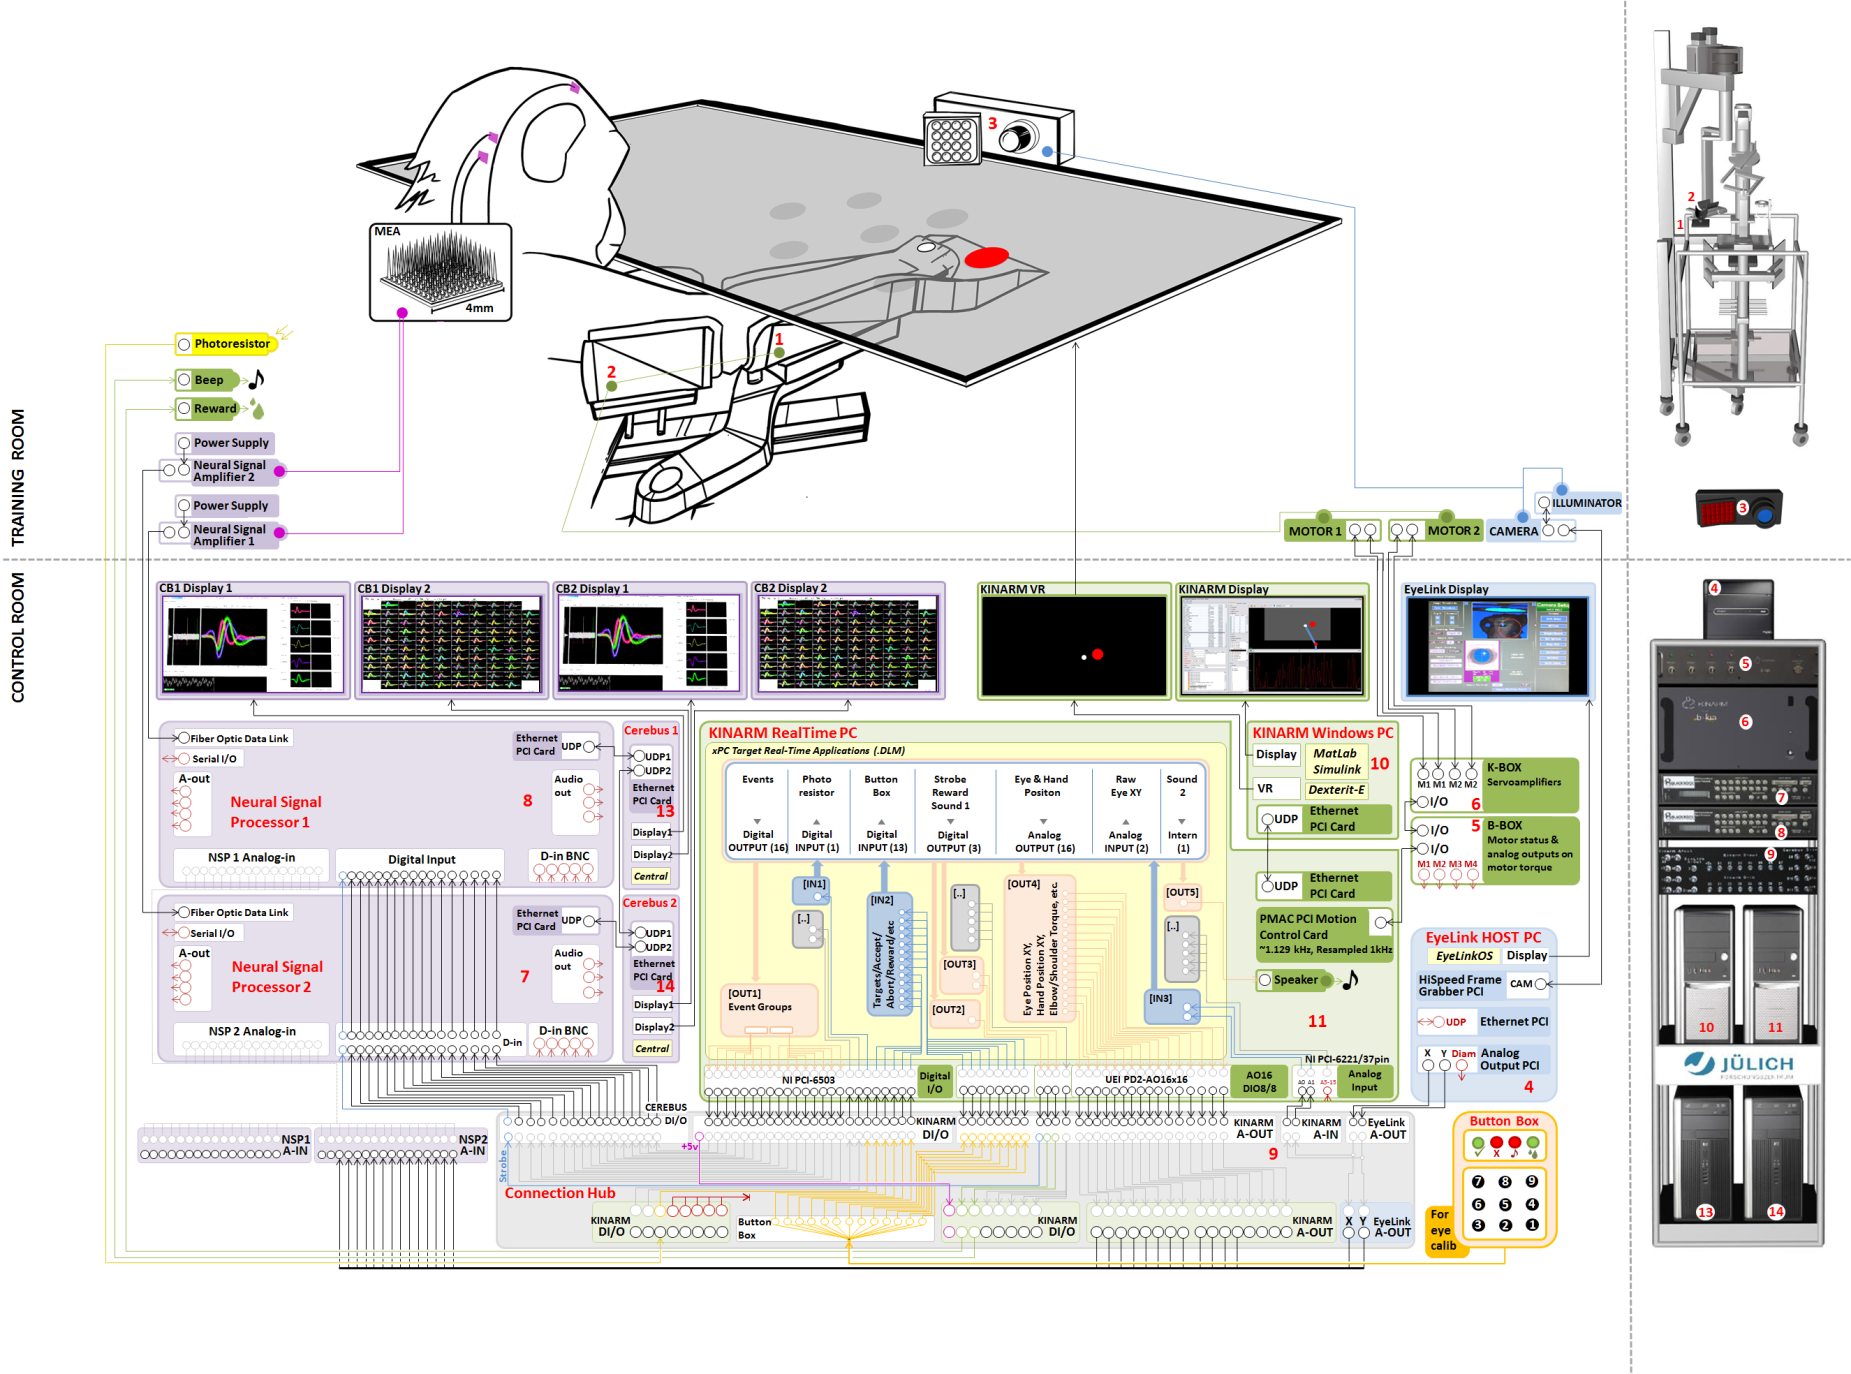
\includegraphics[width=0.8\textwidth]{figures/workflows/river_setup_hardware}
 \caption[The RIVER setup]{The RIVER setup including schematic of hardware components and signal flows. Depicted are the monkey task setup (top right), the recording system and signal flows (bottom left), the monkey chair and Kinarm (top right) and the recording hardware rack (bottom right). Figure from \citet{deHaan_2018a}.}
 \label{fig:river_setup}
\end{sidewaysfigure}


\begin{table}[]
\centering
\begin{tabular}{ll}
\hline
file format & content                                               \\ \hline \hline
*.ccf       & cerebus configuration                                 \\ \hline 
*.nev       & digital events                                        \\
            & \textbullet~ unsorted spike times                      \\
            & \textbullet~ spike waveforms                          \\
            & \textbullet~ experiment metadata                      \\
            & \textbullet~ trial metadata                           \\
            & \textbullet~ screen events                            \\
            & \textbullet~ exoskeleton events                       \\
            & \textbullet~ behavioural events                       \\
            & \textbullet~ errors                                   \\
            & \textbullet~ ...                                      \\ \hline
*.ns2       & continuous signals with $1kHz$ sampling rate           \\
            & \textbullet~ eye (gaze) position                      \\
            & \textbullet~ hand position                            \\
            & \textbullet~ target position                          \\
            & \textbullet~ elbow position                           \\
            & \textbullet~ joint angles / velocities / accelerations \\
            & \textbullet~ synchronization pulses                   \\ \hline
*.n6        & continuous signals with $1kHz$ sampling rate           \\
            & \textbullet~ neuronal signals                         \\ \hline
\end{tabular}
\caption[Recording file formats and content in the Vision-for-Action project]{Recording file formats and content in the Vision-for-Action project. The cerebus configuration is saved in a custom \software{Blackrock} configuration format. The nev format contains digital events generated by the NSP based on the neuronal activity (spike detection) and all integrated events received from additional hardware systems, e.g. the Simulink model. Continuous signals are stored in different files depending on the sampling resolution. At a low sampling resolution of $1kHz$ the ns2 signal contains behavioral signals whereas the neuronal high sampling resolution signals are stored in the ns6 file.}
\label{tab:v4a_recording_files}
\end{table}


As for the Reach-to-Grasp experiment, the \code{nev} file contains online extracted spikes, but in addition it also captures a large amount of structured metadata in form of events, which encode experimental metadata as outlined above.
These metadata are complemented by a set of metadata descriptors. These are text files in \code{csv} format, structured in an \software{odMLtables} compatible fashion. These files are generated by the experimenter in a manual using \software{Matlab} routines for generation of repetitive data. The content of these files contains a structure for metadata branches that can be merged and integrated in an hierarchical \software{odML} metadata collection. A complete set of descriptor files encompasses $9$ \code{csv} files and covers all metadata not captured in the event recording file. These \code{csv} files store essential metadata about the monkey, the hardware components used, the global and specific codes used in the session, the signal flow for digital and analog signals in the recording setups and the general description of the recording session as well as meta information about all required descriptor files (\cref{tab:v4a_metadata_files} top). Additionally, configuration and supplemental files that can not be captured in a csv file but are used during the recording are referenced in the session descriptor. Most of the metadata files are expected to be identical for all sessions. Some on the other hand change with the task type, while only a few need to be generated / tracked explicitly for each session. Nevertheless, since during the life time of an experiment unforeseen changes might occur, such as the replacement of a part of the setup due to malfunction, it is better practice to record all metadata files anew in each session regardless of prior expectations. We also followed this approach in this specific experiment.
% \todo{add example for descriptor in paragraph above?}

\begin{table}[]
\scriptsize
\centering
\begin{tabular}{lll}
\textbf{Descriptor}                                & \textbf{Content}                                                                                                       & \textbf{Generation}                                                                  \\ \hline \hline
\multicolumn{1}{l}{session}                      & \multicolumn{1}{l}{\textbullet~ session name}                                                                         & \multicolumn{1}{l}{once per session}                                                \\
\multicolumn{1}{l}{}                             & \multicolumn{1}{l}{\textbullet~ relevant metadata files}                                                              & \multicolumn{1}{l}{semi-automatic}                                                  \\
\multicolumn{1}{l}{}                             & \multicolumn{1}{l}{\textbullet~ task type}                                                                            & \multicolumn{1}{l}{visual cross check}                                              \\
\multicolumn{1}{l}{}                             & \multicolumn{1}{l}{\textbullet~ ...}                                                                                  & \multicolumn{1}{l}{}                                                                \\ \hline
\multicolumn{1}{l}{subject}                      & \multicolumn{1}{l}{\textbullet~ species}                                                                              & \multicolumn{1}{l}{onetime, static}                                                 \\
\multicolumn{1}{l}{}                             & \multicolumn{1}{l}{\textbullet~ active hand}                                                                          & \multicolumn{1}{l}{}                                                                \\
\multicolumn{1}{l}{}                             & \multicolumn{1}{l}{\textbullet~ training}                                                                             & \multicolumn{1}{l}{}                                                                \\
\multicolumn{1}{l}{}                             & \multicolumn{1}{l}{\textbullet~...}                                                                                   & \multicolumn{1}{l}{}                                                                \\ \hline
\multicolumn{1}{l}{Kinarm}                       & \multicolumn{1}{l}{\textbullet~ hardware specifications}                                                              & \multicolumn{1}{l}{onetime, static}                                                 \\
\multicolumn{1}{l}{}                             & \multicolumn{1}{l}{\textbullet~ programming software}                                                                 & \multicolumn{1}{l}{}                                                                \\
\multicolumn{1}{l}{}                             & \multicolumn{1}{l}{\textbullet~ ...}                                                                                  & \multicolumn{1}{l}{}                                                                \\ \hline
\multicolumn{1}{l}{eyelink}                      & \multicolumn{1}{l}{\textbullet~hardware specifications}                                                               & \multicolumn{1}{l}{onetime, static}                                                 \\
\multicolumn{1}{l}{}                             & \multicolumn{1}{l}{\textbullet~ software specifications}                                                               & \multicolumn{1}{l}{}                                                                \\
\multicolumn{1}{l}{}                             & \multicolumn{1}{l}{\textbullet~ ...}                                                                                  & \multicolumn{1}{l}{}                                                                \\ \hline
\multicolumn{1}{l}{blackrock}                    & \multicolumn{1}{l}{\textbullet~ Utah arrays}                                                                          & \multicolumn{1}{l}{onetime, static}                                                 \\
\multicolumn{1}{l}{}                             & \multicolumn{1}{l}{\textbullet~ connectors}                                                                           & \multicolumn{1}{l}{}                                                                \\
\multicolumn{1}{l}{}                             & \multicolumn{1}{l}{\textbullet~ physical properties}                                                                  & \multicolumn{1}{l}{}                                                                \\
\multicolumn{1}{l}{}                             & \multicolumn{1}{l}{\textbullet~ ...}                                                                                  & \multicolumn{1}{l}{}                                                                \\ \hline
\multicolumn{1}{l}{analog\_communication}        & \multicolumn{1}{l}{\textbullet~ hardware specifications}                                                              & \multicolumn{1}{l}{onetime, static}                                                 \\
\multicolumn{1}{l}{}                             & \multicolumn{1}{l}{\textbullet~ pin mapping}                                                                          & \multicolumn{1}{l}{}                                                                \\
\multicolumn{1}{l}{}                             & \multicolumn{1}{l}{\textbullet~ ...}                                                                                  & \multicolumn{1}{l}{}                                                                \\ \hline
\multicolumn{1}{l}{digital\_communication}       & \multicolumn{1}{l}{\textbullet~ hardware specifications}                                                              & \multicolumn{1}{l}{onetime, static}                                                 \\
\multicolumn{1}{l}{}                             & \multicolumn{1}{l}{\textbullet~ pin mapping}                                                                          & \multicolumn{1}{l}{}                                                                \\
\multicolumn{1}{l}{}                             & \multicolumn{1}{l}{\textbullet~ ...}                                                                                  & \multicolumn{1}{l}{}                                                                \\ \hline
\multicolumn{1}{l}{codes\_global}                & \multicolumn{1}{l}{\textbullet~ code mapping \& definition}                                                           & \multicolumn{1}{l}{onetime, static}                                                 \\ \hline
\multicolumn{1}{l}{codes\_task}                  & \multicolumn{1}{l}{\textbullet~ mapping of global codes to}                                                           & \multicolumn{1}{l}{once per task type}                                              \\
\multicolumn{1}{l}{}                             & \multicolumn{1}{l}{\hspace{1cm} task specific metadata}                                                               & \multicolumn{1}{l}{static}                                                          \\ \hline \\
\textbf{Additional metadata files}                 &                                                                                                                        &                                                                                      \\ \hline \hline
\multicolumn{1}{l}{task description (pdf)}       & \multicolumn{1}{l}{\begin{tabular}[c]{@{}l@{}}extensive human readable task description\\ with sketches\end{tabular}} & \multicolumn{1}{l}{\begin{tabular}[c]{@{}l@{}}once per task,\\ static\end{tabular}} \\ \hline
\multicolumn{1}{l}{task model (mdl)}             & \multicolumn{1}{l}{model description file as used by Simulink}                                                        & \multicolumn{1}{l}{\begin{tabular}[c]{@{}l@{}}once per task,\\ static\end{tabular}} \\ \hline
\multicolumn{1}{l}{task parameter file (dtp)}    & \multicolumn{1}{l}{task parameter file as used by Simulink}                                                           & \multicolumn{1}{l}{\begin{tabular}[c]{@{}l@{}}once per task,\\ static\end{tabular}} \\ \hline
\multicolumn{1}{l}{target picture (png)}         & \multicolumn{1}{l}{image used for visual targets}                                                                     & \multicolumn{1}{l}{onetime}                                                         \\ \hline
\multicolumn{1}{l}{calibration parameters (mat)} & \multicolumn{1}{l}{parameters of the calibration model}                                                               & \multicolumn{1}{l}{onetime}                                                         \\ \hline
\multicolumn{1}{l}{calibration data (mat)}       & \multicolumn{1}{l}{data used for calibration}                                                                         & \multicolumn{1}{l}{once per calibration}                                            \\ \hline
\end{tabular}
\caption[Metadata files in the Vision-for-Action project]{Metadata descriptors and supplementary files in the Vision-for-Action project. Nine \code{csv} descriptor files are required for a complete description of the experiment. Most of these only need to be generated once as the data contained within is constant across consecutive recording sessions. Only the session descriptor needs to be adjusted to each session. There are six additional files which provide supplemental metadata information, e.g. additional configuration and image material used during the recording.}
\label{tab:v4a_metadata_files}
\end{table}

\section{Metadata workflow in the Vision-for-Action project}

Based on the metadata source files described in \cref{tab:v4a_metadata_files} (descriptors, in addition to a number of supplemental and binary data files) we designed a workflow for metadata collection and enrichment which consists of processing steps that can be classified into five processing categories (\cref{fig:v4a_metadata_workflow_rulegraph}). In the following, we present concepts and implementations developed for in the context of Vision-for-Action. We design the workflow using snakemake in combination with Python scripts, which are implemented in a standalone fashion as described in \cref{sec:snakemake} (\cref{code:workflows_python_scripts}). In the context of this workflow we term these standalone Python scripts 'application' (app). Each app performs only a single, designated processing step based on as few input files as possible, to avoid unnecessary dependencies and provide a processing workflow that is easy to follow.

\paragraph{Grouping of apps}
We separated apps into groups according to the similarity of their interfaces, i.e. the input parameters the app requires and the type of output it generates. This way a single rule can handle multiple apps in case they have a similar dependency structure and require the same parameters. An example for a group of app with the same interface are metadata apps, coordinated by the \code{run\_metadata\_app} rule (\cref{fig:v4a_metadata_workflow_rulegraph}, green box). This rule covers all apps, which generate metadata based on the original recording data and generate an \software{odMLtables} compatible csv file summarizing the extracted metadata or processing results. These apps require as input parameters the location of the original data files to be loaded as well as the location to which to write the resulting \code{csv} file. In contrast to this \code{data\_apps} extend the original data (in the \software{Neo} representation) and generate an \software{odMLtables} compatible \code{csv} file. Each generated \code{csv} file is saved with an app-specific filename and typically contains only a few values of additional metadata, since apps are modularized to cover very specific tasks.
In the current workflow, metadata and data apps are implemented in a flexible manner, as these apps are located in a dedicated folder. All apps in these folders are automatically included in the workflow and are executed by the \code{run\_metadata\_app} and \code{run\_data\_app} rules (\cref{code:v4a_workflow_snakemake_rule}).
% \todo{add concrete examples for this type of app.}

Two minimal examples depicting two subsets of the workflow are shown in \cref{fig:v4a_metadata_workflow_dag}. Here we focus on the integration of the original \code{csv} descriptors into a single \software{odML} file as well as the execution of preprocessing steps (\cref{fig:v4a_metadata_workflow_dag}A and B, respectively). The general dependencies between the corresponding rules are visible in \cref{fig:v4a_metadata_workflow_rulegraph}, whereas the executions of the rule with varying parameters during a run of snakemake are depicted in \cref{fig:v4a_metadata_workflow_dag}. I.e. the two rules handling data and metadata apps (\cref{fig:v4a_metadata_workflow_rulegraph}, green boxes) each cover a multitude of data and metadata apps. Examples of the apps run by these two rules are depicted in (\cref{fig:v4a_metadata_workflow_dag}B), e.g. the \code{run\_data\_app} rule executes the apps \code{app\_synchrofact\_detection}, \code{app\_cross\_talk\_detection\_in\_ns6} and \code{app\_saccade\_detection} all with the same set of parameters. The large number of apps handled by some of the rules prevents a visualization of the complete workflow in this context, hence only a small selection of apps is depicted \cref{fig:v4a_metadata_workflow_dag}.

\begin{figure}
    \centering
    \includesvg[width=\textwidth, pretex=\relscale{0.7}]{./figures/workflows/rulegraph_colored_escus}
    \caption[Metadata workflow rules for Vision-for-Action experiment]{Metadata workflow rules for Vision-for-Action experiment. Visualized are only the general dependencies between rules irrespective of the input parameters and multiple executions during the run of the workflow. Data are preprocessed (green boxes) and secondary metadata are extracted. These are together wit the primary metadata are combined in a single metadata collection (blue boxes). Data are converted to the \software{Nix} format and packaged together with the metadata in a single file (purple boxes). The resulting files are then put under version control using \code{gin} and uploaded to a central server (yellow boxes).}
    \label{fig:v4a_metadata_workflow_rulegraph}
\end{figure}


\begin{sidewaysfigure}
    \textbf{A}\\
    \scalebox{0.85}{
    \includesvg[width=\textwidth, pretex=\relscale{0.05}]{./figures/workflows/v4a_dag_all_descriptors_mod_escus}}\\
    \textbf{B}\\
    \scalebox{0.85}{
    \includesvg[width=\textwidth, pretex=\relscale{0.01}]{./figures/workflows/v4a_dag_all_apps_mod_escus}\\}
    \caption[Metadata workflow examples from Vision-for-Action experiment]{Two example metadata workflow steps in the Vision-for-Action project. \textbf{A)} Integration of original \code{csv} descriptors into a single \software{odML} file by repeated application of the \code{copy\_descriptors} and \code{csv\_to\_odml} rule. Each application is specific for a single descriptor and resulting \software{odML} files are merged via the \code{integrate\_descriptors} rule. A style sheet is automatically downloaded for easy visualization of the generated \software{odML} files.\textbf{B)} Preprocessing and metadata extraction via repeated application of the \code{run\_data\_app} and \code{run\_metadata\_app} rule. Both rules have similar parameter sets, but \code{run\_data\_app} additionally depends on an extendable version of the original recording data structure, which is generated by the \code{data\_to\_nix} rule. The rules take as parameter the app to run and the recording session. All rules above are triggered by a utility rule requiring the output files of all preprocessing apps as input.}
    \label{fig:v4a_metadata_workflow_dag}
\end{sidewaysfigure}


\begin{codeenv}
\inputminted[firstline=149, lastline=164, linenos,tabsize=2,breaklines, fontsize=\scriptsize]{bash}{figures/workflows/v4a_workflow.snakefile}
\caption[Excerpt of the snakemake workflow definition for the Vision-for-Action project]{Excerpt of the snakemake workflow definition for the Vision-for-Action project. The \code{run\_metadata\_app} rule requires all apps located in the \code{metadata\_app} subfolder as well as the locations of the original dataset and the utility functions for this workflow. It generates a \code{.done} file with an app specific name for housekeeping purposes as well as a \code{csv} file containing the extracted metadata. The execution environment is defined via a conda environment. The rule executes three lines of bash code for making the utility functions available, running the app with the specific parameters and generating / updating the housekeeping \code{.done} file. The variables \code{DATALOC}, \code{OUTPUTLOC} and \code{UTILDIR} are fixed path locations within the snakemake workflow and either defined via the configuration or are set at the beginning of the workflow description.}
\label[codelisting]{code:v4a_workflow_snakemake_rule}
\end{codeenv}

In the first example, covering the merge of descriptors, first all \code{csv} descriptors need to be copied to the working directory of the workflow as the descriptors are stored together with the original data in a read-only folder. This prevents unintentional changes of the original data and makes the workflow less error-prone. Each descriptor file is copied by the \code{copy\_descriptors} rule whereas the descriptor identity is defined as parameter. These copies serve as an input for the \code{csv\_to\_odml} rule, which permits the conversion of any \software{odMLtables} compatible \code{csv} file to the \software{odML} format. This step is also run for all descriptors separately. In addition the \code{csv\_to\_odml} rule also requires an \software{odML} style sheet for the user friendly visualization of the \software{odML} file via \code{html}. This is a required input file for all realizations of the \code{copy\_to\_csv} rule and is downloaded once to the descriptor working directory via the \code{add\_odML\_style\_sheet} rule. Finally, the \code{integrate\_descriptors} rule uses all previously created \software{odML files} as input and integrates all \software{odML} files into a common \software{odML} file.

In the second example, two types of preprocessing steps are performed: preprocessing and metadata extraction with and without modification or extension of the neuronal data set. Apps that only access the original neuronal data to extract metadata (e.g. data integrity checks) are coordinated by the \code{run\_metadata\_app} and access the neuronal data in the original \software{Blackrock} format. Preprocessing steps that extend the original neuronal dataset (e.g. by performing spike sorting) are handled by the \code{run\_data\_app} rule and require a data representation in the generic, open source \software{Nix} format (see \cref{sec:nix_format}), to be able to successively extend the dataset. The initial conversion from the \software{Blackrock} to the \software{Nix} format is performed by the \code{data\_to\_nix} rule. Here, the order of execution of the data apps is not specified in the snakemake workflow as there are no dependencies between the different runs of the \code{run\_data\_app} rule. Hence the order of execution depends on the snakemake run and is not predetermined. This means only independent data processing steps can be implemented with this mechanism as no fixed order is guaranteed. Future extensions adding interdependent preprocessing steps can be added as additional rules in the snakemake workflow by assigning the new rules with a higher rule priority order than the \code{run\_data\_app} rule (see \cref{code:workflows_simple_snakefile}, line 1-3) and introducing additional, explicit dependencies to other rules.

Currently, metadata apps cover aspects of data quality assurance as well as extraction of essential information for easy access. Some examples for data quality assurance apps are listed below:
\begin{itemize}
 \item check for the existence of all recording files
 \item check for the integrity of events recorded with both NSP systems. This ensures synchronicity of the datasets between the two independent \software{Blackrock} recording systems.
 \item check for integrity of online extracted spikes and continuously sampled raw data. In case of a silent data packet loss during the recording, online extracted spike times and continuous data are not aligned from the time point of data loss (see also \cref{sec:additional_features_gaps}). The occurrence of a gap can be automatically detected with a high probability by comparing online generated spiking event times to the continuous recording signal at high sampling rate.
\end{itemize}

Examples for apps for the automatic extraction of basic metadata are:
\begin{itemize}
  \setlength{\itemsep}{0pt}
  \setlength{\parskip}{0pt}
  \setlength{\parsep}{0pt}
 \item the collection of all channel specific information in a channel-specific \software{odML} \code{Section}.
 \item the evaluation whether a session was offline spike sorted
 \item the evaluation of the monkey's performance (total number of trials, number of correct trials)
 \item the creation of overview plots of 
 \begin{itemize}
  \setlength\itemsep{0pt}
  \setlength{\parskip}{0pt}
  \setlength{\parsep}{0pt}
  \item the raw recorded data for the purpose of visual inspection
  \item detected hyper-synchronous events in the spiking data and their complexity distribution (see \cref{sec:spike_data_quality})
 \end{itemize}
\end{itemize}

In contrast to metadata apps, data apps extend the \software{Neo} data structure. Some examples of implemented and envisioned data apps are:
\begin{itemize}
  \setlength{\itemsep}{0pt}
  \setlength{\parskip}{0pt}
  \setlength{\parsep}{0pt}
 \item the detection of cross talk between individual electrodes and annotation of the corresponding recording traces
  \item the detection and annotation of hyper-synchronous events in spiking data (see \cref{sec:spike_data_quality})
 \item the extraction of events from continuous recording signals such as
 \begin{itemize}
  \setlength\itemsep{0pt}
  \setlength{\parskip}{0pt}
  \setlength{\parsep}{0pt}
  \item the extraction of saccades from the eye (gaze) position
  \item the segmentation of the hand movement into sub-trajectories
 \end{itemize}
\end{itemize}


\paragraph{Code and data folder structure}
The workflow project is organized in the following structure:\\

\renewcommand*\DTstylecomment{\color{gray}\textit}
\renewcommand*\DTstyle{\textcolor{black!90}}
\begin{minipage}[t]{\textwidth}
\dirtree{%
.1 workflow folder\DTcomment{workflow repository folder}. 
.2 Snakefile\DTcomment{definition of snakemake workflow}.
.2 config.yaml\DTcomment{configuration of snakemake workflow}.
.2 config\_template.yaml\DTcomment{template for setting up config.yaml}.
.2 envs.
.3 metadata\_env.yaml\DTcomment{contains conda Python environment definitions}.
.2 scripts\DTcomment{contains Python scripts coordinated by snakemake}.
.3 data\_apps\DTcomment{contains modifying/extending data apps}.
.3 metadata\_apps\DTcomment{contains aggregating metadata apps}.
.3 infrastructure\DTcomment{contains general purpose apps}.
.3 utilities.
.4 util.py\DTcomment{contains utility functions used by apps}.
.3 tests\DTcomment{contains test suite for apps}.
.3 app\_example.py\DTcomment{template implementation of an app}.
}
\ \\
\end{minipage}

The separation of different types of apps into subfolders permits to automatically collect data and metadata applications during the runtime of the snakemake workflow. This avoids hard coding of app names in the workflow definition and provides a more flexible approach that minimizes the need for the user to customize the Snakefile.
Within the snakemake workflow, different paths need to be configured via the \code{config.yaml}: i) the location of the original data files, typically only with read access, ii) the output location of the workflow, iii) potentially the server repository the results will be uploaded to. In addition to this, the configuration file can be used to specify a set of recording sessions to run the workflow on. Otherwise all available data folders will be used by default.
Within the snakemake workflow, multiple folders are used to separate data and metadata at different levels of processing:\\

\begin{minipage}[t]{\textwidth}
\dirtree{%
.1 <session>\DTcomment{session specific data and metadata workflow folder}. 
.2 <session>\_original.nix\DTcomment{data as contained in \software{Blackrock} files descriptors}.
.2 <session>.nix\DTcomment{processed and extended data and metadata}.
.2 <session>\_small.nix\DTcomment{slim version of the <session>.nix file (no raw data)}.
.2 metadata\_complete.odml\DTcomment{metadata from descriptors and preprocessing}.
.2 app\_results\DTcomment{contains metadata output from preprocessing}.
.3 preprocessing\_integrated.odml\DTcomment{all metadata from preprocessing}.
.3 csvs\DTcomment{contains csvs generated by preprocessing steps}.
.3 odMLs\DTcomment{contains csvs converted to odML format}.
.2 app\_stats\DTcomment{contains files indication the execution status of apps}.
.2 descriptors\DTcomment{contains descriptor processing steps}.
.3 csvs\DTcomment{contains data related to csv descriptors}.
.3 odMLs\DTcomment{contains csv descriptors converted to odML format}.
.4 descriptor\_session\_integrated.odml\DTcomment{all descriptor metadata}.
}
\ \\
\end{minipage}








\paragraph{Metadata aggregation (data \& metadata apps)}
Primary, initial metadata are available as \software{odMLtables} compatible \code{csv} descriptors. Secondary, automatically extracted metadata are generated in the same format by a number of preprocessing steps implemented as \code{metadata} and \code{data} apps (\cref{fig:v4a_metadata_workflow_rulegraph} green boxes). Both sets of \code{csv} files are converted into the \software{odML} format using the generic \code{csv\_to\_odml} rule which is based on \software{odMLtables}. In a two level approach, first metadata information originating from descriptors and preprocessing steps are each merged into single \software{odML} files. In a second step, these are integrated into the complete metadata collection for the given recording session (\cref{fig:v4a_metadata_workflow_rulegraph}, blue boxes).

\paragraph{Data packaging}
The original data are stored in a \software{Blackrock} binary data format, which is optimized for the recording of large data streams. To access, analyze and modify/extend the data we use the open-source \software{Nix} format which is based on the  \code{hdf5} standard and offers a direct interface to the Python \software{Neo} package. Hence, all data processing and extension apps are based on a data representation in the \software{Nix} format, which is generated by the \code{data\_to\_nix} rule (\cref{fig:v4a_metadata_workflow_rulegraph}). This representation is then firstly extended by a number of data preprocessing apps (\code{run\_data\_app} rule) and secondly merged with the complete metadata collection (\code{integrate\_metadata} rule). Next, links between the data and metadata within the \software{Nix} file are established, connecting \software{Neo} objects to the corresponding sections of the metadata collection (\code{link\_metadata}). To provide appropriately sized packaged data for different analysis purposes, we define two flavours of \software{Nix} files: a \code{full} flavour, containing the complete dataset and a \code{small} flavour containing only memory friendly spiking activity and metadata.

\paragraph{Versioning \& deployment}
We envision the automatic tracking of final metadata and data files generated by the presented workflow using a version control system capable of handling large data files (\cref{fig:v4a_metadata_workflow_rulegraph}, orange rules). We investigate the integration with \software{Gin} web service for hosting data, since it is based on the common versioning software stacks \software{git}\footnote{git, \url{https://git-scm.com}} and \software{git-annex}\footnote{git-annex, \url{https://git-annex.branchable.com/}}. This requires the configuration of a local and optionally remote repository including access right handling. Automatic versioning and remote hosting of results from the snakemake workflow guarantees the consistency of datasets across time. Additionally, the snakemake workflow itself can also be tracked in the same repository, assuring a direct link between the workflow result and the contributing source code.
Another advantage of hosting the packaged data files remotely is the central storage, providing a single reference location for all scientists working with the data. At the same time the version control system permits easy and clear communication about the data and the up-to-dateness is ensured via the automatic registration of results from the snakemake execution.
We found that for a one directional interaction in which snakemake is only adding results to the repository, the integration of the two systems works smoothly. Potential problems occur in cases when the version control system is used to check out files which act as input files to any rule in the workflow. Here, the modification time stamp of the file is not conserved between registration in the version control system and the time point of check out. However, since snakemake relies on consistent modification timestamps of files for the status of the workflow, this can lead to inconsistencies in the workflow management.

\paragraph{Validation}
Modularization of the individual processing steps into apps permits the implementation of validation routines to ensure correct functionality of the code. Since in this experiment the apps are Python based, tests can be implemented e.g. via the \code{unittest}\footnote{unittest, \url{https://docs.python.org/3.7/library/unittest.html}} framework. Combining this concept with a versioned data repository, such test could be integrated with one of the available continuous integration systems (see \cref{sec:r2gpipeline_evaluation}), which automatically trigger validation routines on each code update.

\subsection{Discussion}
Based on the concepts we described above, we implemented a prototype of the data processing workflow. Here, we discuss the individual features exhibited by this approach and contrast it to the workflow implemented for the Reach-to-Grasp project (\cref{sec:data}).

\label{sec:workflow_discussion}
\paragraph{Efficiency \& reliability}
By implementing the workflow in snakemake, inherently only those workflow steps are executed for which updated input files exist. This reduces the amount of overhead and execution time in comparison to a non-modular, scripted, rigid workflow for which all steps can only be executed at once without taking into account intermediate results.
At the same time using snakemake for determining which steps need to be re-executed is a much more reliable approach in comparison to manual evaluation of the up-to-dateness of intermediate results and initialization subsequent processing steps.

\paragraph{Flexibility \& usability}
Already during the early development and installation of the workflow, output files can be generated (e.g. the complete metadata collection in \software{odML} format or the recording data in \software{Nix} format) even if they do not yet contain all information. These preliminary output files will grow proportional to the information contained by the continued extension of the workflow definition. This permits to provide output files to the collaboration community according to the software development philosophy \textit{'Release early, release often'} \citep{Martin_2008} already at early implementation stages. At the same time the modular structure and simple definition of the workflow in a snakemake file permit a flexible extension of the procedure also at later time points during the production, e.g. when a new method for data quality estimation is developed and should be applied to all previously recorded sessions. In simple cases this can be achieved by adding an new app to the \code{data} or \code{metadata} apps folder, which will be automatically considered in the next workflow run, thus making maintenance of the workflow easy. For more complex changes, which require additional steps in the workflow process, new rules can be added, which will be automatically integrated based on their \code{input} and \code{output} file dependencies.

\paragraph{Reusability}
The presented workflow rules and apps can be grouped into two categories: Those which do require some knowledge about specific aspects of the project and those which only require general information about file formats and generic tools. An  example for the first group is the app linking between the data and the metadata part within a \software{Nix} file (\cref{fig:v4a_metadata_workflow_rulegraph}, \code{link\_metadata} rule). This rule requires information about the data structure and its interpretation as well as about the metadata originating from the \software{odML} file to be able to draw semantically useful links between the two. Another example are the various \code{metadata} apps, which need to be able to identify the relevant information in the source data files to interpret and extract this into a \code{csv} file.
On the other hand, other apps and rules are generic. For example, the conversion from \code{csv} to the \code{odML} format does not require information about the actual file content. Other examples for generic rules are the integration of multiple \software{odML} files into a single file (\code{integrate\_descriptors\_and\_app\_results} rule), the integration of \software{odML} into \software{Nix} (\code{integrate\_metadata} rule) or the setup of the \software{gin} repository. Thus a large amount of apps can be reused across projects, lowering both effort and cost of setting up data management workflows  and making processed datasets more similar from different experiments.

\paragraph{Robustness}
Robustness of the workflow is strengthened in the modularity of the snakemake rules: In case one of the rules fails to produce the expected output files, e.g. by encountering invalid or unexpected data, snakemake keeps intermediate files. This permits to generate output files under erroneous conditions without explicitly handling all possible exceptions in the individual apps.

\paragraph{Outlook}
We plan to extend the existing workflow at multiple points. Firstly, on the side of \code{data} and \code{metadata} apps, there are a number of  steps for preprocessing and information extraction which would simplify data selection for later analysis. This includes for example the definition of trials already in the preprocessing stage to provide a unified trial framework for all collaborators. Similarly, the calculation of common measures of spike train statistics can be performed at that stage and shared between scientists. Additional approaches for data quality assurance are the automatic detection of noise in raw signals and the detection of cross talk between electrodes using a coherency approach. Furthermore, additional metadata not covered by descriptors can be extracted from supplementary files and be added to the metadata collection. A more ambitious, but realistic extension would be to introduce an additional, automatic spike sorting based on the raw recording traces, which can be evaluated against the spike sorting version if manual sorting was performed for the specific session. 

Secondly, in case of sequential dependencies between the extensions discussed above, additional, explicit rules for handling these need to be added in the workflow and a rule order needs to be defined for the disambiguation of the new and existing \code{data} and \code{metadata} rules.

Thirdly, the separation of generic from experiment specific apps into a separate Snakefile would highly increase the reusability of the workflow. This utility Snakefile could be integrated in multiple projects as generic rules can be reused in different contexts. Sharing these snakemake rules and apps would optimally occur via a separate repository or package collecting general purpose workflow functionality wrapped by snakemake rules.

Fourthly, with respect to the different needs for archival of intermediate and final workflow results, the structure of the output can be adjusted to reflect whether the respective content requires archival. An example for the separation on top of the existing folder structure could be as follows: a source folder containing a copy of the original source data and metadata files, a cache folder for all intermediate and volatile files as well as an output folder containing all user relevant results of the workflow (final \software{odML} and annotated \software{Nix} files). Thus the cache folder can be removed if required.

Fifthly, to exploit snakemake capabilities, the workflow should run in parallel on a compute cluster. With snakemake supporting common queuing systems, it facilitates the migration from a local, serial implementation of the workflow towards a parallelized execution on a high performance cluster. As the amount of data increases, such compute power is becoming a necessity.

\paragraph{Future challenges}
% timestamp issue with snakemake and gin
The integration of a file modification timestamp based WMS with a version control system where modified files are based on hashes is not straightforward. Version control systems like git do not track the original modification time stamp of a file, but instead update the timestamp every time they modify the file representation on disc. This can lead to inconsistencies in the workflow management of snakemake if a version control system was used to checkout files. In the presented workflow scenario this is not an acute problem, since gin is only used to capture the content of all files of the workflow once at the end of the generation process and not to review older versions of the files. A workaround for avoiding version control and workflow management interference would be to additionally track the original modification time stamp of files and restore this information upon checkout.

% additional overhead via repetetive loading \& saving
The input and output file based workflow description as implemented by snakemake leads to frequent reading and writing of data, which could be prevented in a monolithic workflow implementation in a single script, as presented in \cref{sec:r2g_preprocessing_pipeline}. Here, the workflow management increases the overhead of data preprocessing. However, there are multiple factors which can counteract or attenuate this effect: i) the usage of efficient reading and writing routines, ii) the reading of only the required part of the data and iii) the workflow management itself, as it only executes required workflow rules. Since snakemake is already handling the workflow in an optimized fashion, the most potential for improvement lies in the read and write routines in terms of efficiency and loading of specific data. 

% how to handle utility files in snakemake?
The current snakemake workflow implementation features a utility script, which contains centralized functionality needed by multiple apps (e.g. read and write data to \software{Nix} or \code{csv}). This script is therefore a required input file for a multitude of rules, and it stated explicitly in all \code{input} declarations. This duplicated code is not conform with the common software development principle \textit{'Don't repeat yourself'} \citep{Martin_2008}. However, within the framework of snakemake up to now, there is no satisfying solution for this except to explicitly list the utility script (see \cref{code:v4a_workflow_snakemake_rule}). 

% automatic workflow tiggrering on gin
Version control was introduced to track changes with each execution of the workflow. However, also hosting the original source files in a version controlled environment has advantages. For example, changes in the source files can automatically trigger the workflow and therefore form a fully automated system to update the packaged data upon updates in the source files. However, the original source files and packaged data should be hosted in two separate repositories as the read and write access to the first one should be much stricter than for the second one. This would require the repository of the original source files to trigger the snakemake workflow to build a packaged version of the data and commit it to the second repository. The concept is the same as for continuous integration platforms for software testing, with the only difference of the size of data files handled. Therefore existing systems can potentially be modified to serve this modified purpose. A pilot study investigating the integration of \software{snakemake} workflows into the \software{GIN} system started in June 2019\footnote{\url{https://github.com/G-Node/gin-proc}}.


\subsection{Workflow evaluation}
We evaluate the presented snakemake workflow with respect to the essential requirements for metadata management workflows in complex, collaborative projects defined in \cref{sec:metadata_requirements}. An overview of the evaluation can be found in \cref{tab:requirement_check_v4a}.

The presented workflow uses \software{odML} as a basis for metadata structuring. By using the \software{odML} framework, common terminologies are automatically defined when setting up the \software{odML} document (\requirement{R1}). This also automatically makes the metadata collection machine and human readable (\requirement{R2}), as \software{odML} is \code{xml} based and offers user-friendly tools for comprehensive visualization (\software{odMLtables}, odML-UI, odml\_view).

We discussed potential extensions of the workflow including the automatic registration of workflow results at a central server. The combination of the presented workflow with such a remote repository can also be used to host the workflow definition and included scripts (\requirement{R4}). This can be achieved by extending the local tracking of versions, e.g. using \code{git} and \code{git-annex}, by a remote server, e.g. the \software{GIN} web service (\requirement{R3}). In combination with a fully automatized workflow (\requirement{R5}), the packaged data and additional output files can be added automatically to a centralized repository and this way made immediately accessible to all collaboration partners.

The presented workflow does not require manual interaction during the execution and automatically executes only required workflow steps, improving the efficiency and making the workflow less error-prone than a manual execution (\requirement{R5}). In case manual preprocessing steps can not be avoided, e.g. for supervised spike sorting, the generated files enter as input files in the workflow. A mechanism for the automatic initiation of a snakemake workflow hosted on \software{GIN} is under development.

The modularization introduced in the workflow by using \software{snakemake} rules and apps makes the workflow highly flexible for future adaption and extensions (\requirement{R6}). Depending on the required change, additional preprocessing scripts only need to be added while the workflow definition itself remains unchanged. Changes involving the adaptation of the workflow can be implemented by introducing additional input and output files, relating new \software{snakemake} rules to existing ones.
Due to the modularization of the workflow, generic and project specific workflow steps can be easily separated making large parts of the workflow reusable in different contexts (\requirement{R7}). The reusability can be further improved by separation of generic rules in a dedicated, public repository.

The workflow can provide complete provenance tracking and reproducibility when integrating all involved files into the version control system. This includes the workflow definition (Snakefile), all files called by the workflow (apps, utility and other Python scripts, configuration files, conda environment definitions), or corresponding version identifiers of these,  as well as the generated output files. In an optimal case this also includes version identifiers of the original, read-only source files. The provenance tracking of Python dependencies can be implemented by specifying exact software versions for the conda environments used for different rules in the workflow or by extracting the current software stack during each run of the workflow (\requirement{R8}).

The workflow generates a compiled version of the data and metadata in a single \software{Nix} file ensuring the consistency of contained data and metadata (\requirement{R10}). Accessing the data only requires a current installation of the \software{Neo} package, making the data available also to inexperienced users without installation of additional packages or custom scripts like the \code{ReachGraspIO}. This lack of dependencies permits the user to benefit from continuously deployed, packaged data as no additional software requirements are introduced when updating the data. This way the user can exploit being continuously updated on the data and metadata side without suffering from software version inconsistencies.

\software{Nix} is based on the standardized \code{hdf5} format. This makes access to the data more memory efficient. It can also be implemented for other programming languages besides Python. Since data and metadata are linked, it makes it easy for users who are not familiar with the metadata structure to access the metadata of a corresponding data object. (\requirement{R9}).

By building the workflow based on Python, all utilized software packages are open-source (\requirement{R11}). This includes \software{odML} and \software{odMLtables} (\cref{sec:metadata}) for metadata handling, \software{Neo} and \software{Nix} for data representation and storage, and \software{snakemake} for the implementation of the workflow. Additional  canonical Python packages are used in the context of individual apps, like \software{Matplotlib} for visualization as well as \software{NumPy} and \software{SciPy} for efficient array based computation.

\begin{table}[]
\footnotesize
\begin{tabular}{lll}
\hline
Requirement                                          &  \cite{Brochier_2018} & Vision-for-Action \\  \hline
R1: Common terminologies                             &  in project & in project \\ 
R2: Structured machine \& human readable metadata    &  yes & yes \\ 
R3: Central data and metadata location               &  no & planned \\ 
R4: Version control                                  &  no & yes \\ 
R5: Mostly automatic metadata compilation            &  manual initialization & yes \\ 
R6: Extendable metadata workflow                     &  minimal & yes \\ 
R7: Reusability                                      &  partial & yes \\ 
R8: Standardized \& reproducible preprocessing       &  no & yes \\ 
R9: Easy to access data and metadata for non-experts &  partial & yes \\ 
R10: Consistent data and metadata                    &  partial & yes \\ 
R11: Open source tools                               &  mostly & yes \\ \hline
\end{tabular}
\caption[Overview of workflow features for Vision-for-Action project]{Overview of features of the pipeline and workflow applied in the Reach-to-Grasp (\cite{Brochier_2018}) and Vision-for-Action projects based on requirements for data and metadata workflows as defined in \cref{sec:scidata_shortcomings} (extension of \cref{tab:requirement_check_scidata}). The presented workflow fulfills almost all essential requirements for metadata management workflows in complex, collaborative projects.}
\label{tab:requirement_check_v4a}
\end{table}


\section{Summary \& guidelines}
\label{sec:guidelines}
We motivated the need for workflow management tools and introduced appurtenant concepts and implementations. We demonstrated \software{snakemake} as a flexible and lightweight tool for Pythonic make-style workflow description and explained its main features based on two examples. In the next step we introduced the Vision-for-Action experiment as a dataset that exceeds the previous Reach-to-Grasp experiment in size and complexity. We described a workflow to handle data and metadata adhering to the FAIR principles for this complex electrophysiology experiment -- from the original recorded data up to user friendly, comprehensively annotated data packages. We also provided detailed examples, discussed features and limitations as well as future plans and challenges.
The presented workflow implements the FAIR principles, as it makes data and metadata findable as it aggregates a comprehensive metadata collection and combines it with the data in a single, searchable \software{Nix} file using global identifiers. Since  \software{Nix} is a standardized format, the data and metadata can be easily indexed by databases making the complete dataset also findable by other scientists once the dataset, or even only the metadata, is published.
The \software{Nix} format is an open, free and universally implementable format making the data and metadata easily accessible with standard protocols. The data and metadata representation is interoperable, since the description within the \software{Nix} file is self contained and references to related metadata can be added using global identifiers.
Provenance information can be tracked within the workflow and stored together with the data in a versioned repository making, in combination with the comprehensive metadata collection, the data reusable by other scientists.
In addition the workflow implementation provides a foundation for the set up of workflows for other experiments, as generic components were identified and extracted from the workflow. This facilitates the realization of the FAIR principles in future experiments. In addition we abstract general guidelines from the presented workflow to ease the implementation of the FAIR principles for other projects :

\begin{description}
 \item[G1: Plan ahead] Integration and usage of data and metadata is a topic discussed concurrently with the development of an experimental setup. There are typically a number of decisions which can simplify the implementation of the data curation workflow later on, like agreeing on a consistent metadata output format for all hardware components or combining multiple data streams in a single file already in the recording setup instead of realigning and merging these files later during preprocessing steps. Also some time should be spend on the design and structure of the metadata collection to avoid reorganizing metadata in later steps.
 \item[G2: Better more than less] Tracking more metadata than the essential ones will most likely turn out to be a wise choice later on, when irregularities are discovered or suddenly a seemingly unimportant parameters is needed for the investigation.
 \item[G3: Make it explicit] Implement the workflow used for data and metadata management explicitly in a formalized workflow language instead of running scripts manually in a certain order. This will make the workflow i) easier understandable, both for others and oneself at a later time ii) provide an overview of the project iii) document your data provenance and preprocessing
 \item[G4: Modularize] Try to segment the  workflow into independent steps, as this will automatically make the workflow easier to understand and reuse, especially when well documented. Try to separate generic processing steps from project specific aspects to improve reusability.
 \item[G5: Keep it linear] Avoid circular dependencies in the  workflow, as these introduce complex dependency structures and indicate a non-optimal segmentation of data / processing steps. When using \software{snakemake} circular dependencies are innately not permitted.
 \item[G6: Think like a user] Be user friendly. Try to provide the data and metadata in a format that requires as little prior knowledge as possible. This increases the chances that others can and more importantly, will make use of the data. Additionally, it paves the way for publication of the data without too much additional overhead.
 \item[G7: Deploy Continuously] This advice from the agile software development approach may as well be applied in a scientific context. Do not attempt to build the perfect workflow, but provide early on intermediate results to collaborators. This enables them to provide valuable feedback and gives them a chance to work with the data while they are still excited about it. For this version management is a prerequisite, since it is essential to be able to communicate about different versions of the workflow output.
\end{description}
